\documentclass[11pt]{article}

\usepackage[utf8]{inputenc}
\usepackage[T1]{fontenc}
\usepackage{lmodern}
\usepackage[a4paper,margin=2.35cm]{geometry}
\usepackage{microtype}
\usepackage{amsmath,amssymb,amsfonts,mathtools}
\usepackage{graphicx}
\usepackage{booktabs,tabularx,longtable,array,multirow}
\usepackage{enumitem}
\usepackage{xcolor}
\usepackage{hyperref}
\usepackage[nameinlink,noabbrev]{cleveref}
\usepackage{natbib}
\usepackage{fancyhdr}
\usepackage{setspace}
\usepackage{caption}
\usepackage{subcaption}
\usepackage{float}
\usepackage{listings}
\usepackage{url}

\definecolor{deepblue}{RGB}{30,70,110}
\definecolor{softgray}{RGB}{245,246,248}
\definecolor{deepred}{RGB}{145,45,45}
\definecolor{deepgreen}{RGB}{35,105,75}

\hypersetup{
  colorlinks=true,
  linkcolor=deepblue,
  citecolor=deepgreen,
  urlcolor=deepred,
  pdftitle={Synthetic Data in the Age of Scaling},
  pdfauthor={Guillaume Harbonnier},
  pdfsubject={Video analysis and research orientation for MMALS, STRAT-Q and probabilistic test governance}
}

\pagestyle{fancy}
\fancyhf{}
\lhead{Synthetic Data in the Age of Scaling}
\rhead{Video Analysis and Research Orientation}
\cfoot{\thepage}
\setlength{\headheight}{14pt}
\onehalfspacing
\setcounter{tocdepth}{2}
\setcounter{secnumdepth}{3}

\newcommand{\MMALS}{\textsc{MMALS}}
\newcommand{\STRATQ}{\textsc{STRAT-Q}}
\newcommand{\MTP}{\textsc{MTP}}
\newcommand{\Real}{\mathrm{real}}
\newcommand{\AI}{\mathrm{AI}}
\newcommand{\Syn}{\mathrm{syn}}
\newcommand{\E}{\mathbb{E}}
\newcommand{\Prob}{\mathbb{P}}
\newcommand{\R}{\mathbb{R}}
\newcommand{\ind}{\mathbf{1}}

\newenvironment{keyidea}{%
  \begin{center}\begin{minipage}{0.93\textwidth}\color{deepblue}\rule{\linewidth}{0.5pt}\par\vspace{0.3em}\noindent\textbf{Key idea.} }%
  {\par\vspace{0.3em}\rule{\linewidth}{0.5pt}\end{minipage}\end{center}}

\newenvironment{mmalsnote}{%
  \begin{center}\begin{minipage}{0.93\textwidth}\color{deepgreen}\rule{\linewidth}{0.5pt}\par\vspace{0.3em}\noindent\textbf{MMALS orientation.} }%
  {\par\vspace{0.3em}\rule{\linewidth}{0.5pt}\end{minipage}\end{center}}

\newenvironment{cautionbox}{%
  \begin{center}\begin{minipage}{0.93\textwidth}\color{deepred}\rule{\linewidth}{0.5pt}\par\vspace{0.3em}\noindent\textbf{Caution.} }%
  {\par\vspace{0.3em}\rule{\linewidth}{0.5pt}\end{minipage}\end{center}}

\title{\textbf{Synthetic Data in the Age of Scaling}\\
\large A Multilevel Video Analysis and Research Orientation for MMALS, STRAT-Q, Probabilistic Test Governance, and Geometric Learning}
\author{Guillaume Harbonnier\\
\small Independent research note -- MMALS / STRAT-Q programme}
\date{Version 1.0 -- 15 June 2026}

\begin{document}
\maketitle

\begin{center}
\begin{minipage}{0.88\textwidth}
\small
\textbf{Status and provenance.} This document is an independent analytical study of Julia Kempe's public lecture \emph{Synthetic Data -- Friend or Foe in the Age of Scaling?}, delivered in the IHES/CNRS \emph{Mathematics for and by Large Language Models} series. It is not a transcript, not an official summary, and not endorsed by the speaker, IHES, NYU, or Meta. It synthesizes the lecture themes, the cited research papers, and an extended technical discussion connecting them to MMALS, STRAT-Q, probabilistic MTP, Test Data Governance, verifiable evidence, continual learning, and geometric filtering.

\vspace{0.8em}
\textbf{Primary video.} \url{https://www.youtube.com/watch?v=D9x3DT16mGg&list=PLx5f8IelFRgHrJ9W6_fbfO3ahDrXMEIWn}
\end{minipage}
\end{center}

\begin{figure}[H]
\centering

\includegraphics[width=2.6cm]{figures/video_qr.png}
\caption*{QR code to the public video and playlist.}
\end{figure}

\begin{abstract}
The rapid proliferation of AI-generated content changes the assumptions under which neural scaling laws were originally observed. A training corpus is no longer only a sample from human or natural data: it may contain outputs of previous models, pseudo-labels, filtered generations, and recursively transformed evidence. This report develops a multilevel explanation of that transition. A first track is written for a twelve-year-old reader, a second for engineers, and a third for graduate and PhD-level readers. We explain power-law scaling, Zipf distributions, perplexity, the Hutter infinite-memory model, tail cutting and tail narrowing, recursive relabeling, modified scaling laws, grokking under mixed real and synthetic data, kernel ridge analyses of model collapse, and verifier-based synthetic-data bootstrapping. We then translate these results into concrete research orientations for MMALS, where the analogous risk is a functional collapse of hosts, routes, memories, and collaborations; for STRAT-Q and probabilistic Master Test Plans, where evidence volume must be separated from evidence strength; and for Test Data Governance, where lineage, freshness, independence, verification, and tail coverage must accompany every synthetic artifact. The central conclusion is that synthetic data can be useful, especially under data scarcity, but scale alone is insufficient. The relevant object to grow is verified functional support rather than raw sample count.
\end{abstract}

\tableofcontents
\newpage

\section{Résumé exécutif en français}

\subsection{Pourquoi cette conférence est importante}

La conférence de Julia Kempe pose une question devenue structurelle : que deviennent les lois d'échelle lorsque les données utilisées pour entraîner les modèles ne proviennent plus seulement d'humains, de capteurs ou de phénomènes naturels, mais aussi des modèles précédents ? Les lois d'échelle classiques suggèrent qu'en augmentant convenablement les paramètres, les données et le calcul, la perte diminue selon une loi de puissance. Cette lecture a fortement influencé la stratégie industrielle des grands modèles. Or la donnée synthétique modifie la distribution d'apprentissage elle-même.

Le risque central n'est pas seulement une augmentation du taux d'erreur. Il est plus subtil :

\begin{itemize}[leftmargin=*]
  \item la longue traîne des cas rares peut être coupée ou rétrécie ;
  \item certaines compétences peuvent ne plus recevoir les exemples nécessaires à leur maintien ;
  \item des pseudo-labels légèrement biaisés peuvent devenir la vérité de la génération suivante ;
  \item davantage de données peut alors améliorer la précision sur une distribution déjà appauvrie, sans rapprocher le système du réel ;
  \item le mélange de réel et de synthétique peut provoquer des plateaux, puis parfois une généralisation tardive de type \emph{grokking} ;
  \item la vérification indépendante peut transformer une grande quantité de candidats imparfaits en un dataset réellement utile.
\end{itemize}

\begin{keyidea}
Le volume brut ne mesure pas l'information nouvelle. Un million de répétitions corrélées ne vaut pas un million d'observations indépendantes. La grandeur importante devient le \emph{support fonctionnel vérifié} : la partie de la réalité ou des compétences qui reste accessible, représentée et contrôlée.
\end{keyidea}

\subsection{La chaîne conceptuelle de la conférence}

La conférence construit progressivement une démonstration.

\paragraph{1. Scaling laws.} Une erreur peut décroître comme
\[
E(T,d) \approx \left(\frac{T_c}{T}\right)^a + \left(\frac{d_c}{d}\right)^b,
\]
où $T$ est la quantité de données et $d$ la taille du modèle. Une ressource insuffisante devient un goulot d'étranglement.

\paragraph{2. Compétences émergentes.} Certaines performances semblent apparaître brutalement avec l'échelle. Il faut cependant distinguer une vraie transition interne, un seuil statistique et un artefact de métrique discontinue.

\paragraph{3. Distributions à longue traîne.} Le langage suit approximativement une loi de Zipf : quelques éléments sont fréquents, beaucoup sont rares. La difficulté, mesurée par exemple par la perplexité, est elle aussi très asymétrique.

\paragraph{4. Modèle de Hutter.} Un système à mémoire infinie qui ne généralise pas peut déjà produire une loi d'échelle. Il répond correctement si une entrée a déjà été observée et s'abstient sinon. Pour $p(i)\propto i^{-\beta}$, son erreur suit
\[
E_T \asymp T^{-(1-1/\beta)}.
\]
Une belle courbe de scaling ne prouve donc ni raisonnement ni abstraction.

\paragraph{5. Coupure de traîne.} Si un générateur synthétique ne produit que les événements jusqu'au rang $k$, l'erreur devient
\[
E_{\mathrm{test}} \asymp T^{-(\beta-1)/\beta} + k^{-(\beta-1)}.
\]
Le premier terme diminue avec les données ; le second est un plancher lié aux cas absents.

\paragraph{6. Récursion.} Chaque génération synthétique ajoute son propre échantillonnage, son erreur d'approximation et éventuellement son bruit de label. Une suite de modèles peut devenir de plus en plus cohérente avec ses prédécesseurs et de moins en moins juste par rapport à la réalité.

\paragraph{7. Mélange réel/synthétique.} Lorsque le réel est rare, le synthétique peut densifier la partie connue et réduire la variance. Lorsque suffisamment de données réelles diverses apparaissent, elles peuvent réancrer l'apprentissage et restaurer la loi de scaling réelle.

\paragraph{8. Vérification.} Un générateur imparfait peut produire une grande quantité absolue de bons exemples. Si un vérificateur indépendant sait distinguer les bons des mauvais, la boucle
\[
\text{générer} \rightarrow \text{vérifier} \rightarrow \text{filtrer} \rightarrow \text{réentraîner}
\]
peut dépasser les performances du générateur initial.

\subsection{Conséquence pour MMALS}

Pour \MMALS, la donnée synthétique n'est pas seulement du texte ou des images. Le système peut produire ses propres routes, activations d'hôtes, synthèses mémorielles et décisions. Ces traces internes deviennent potentiellement les données de la génération suivante.

Le risque analogue au model collapse est un \emph{collapse fonctionnel} :

\begin{itemize}[leftmargin=*]
  \item un hôte légèrement dominant reçoit davantage de gradient et de replay ;
  \item ses routes deviennent plus fréquentes dans la mémoire ;
  \item les hôtes rares reçoivent moins d'expériences ;
  \item la diversité fonctionnelle diminue alors que la stabilité apparente augmente ;
  \item le système devient simple non parce qu'il a convergé localement, mais parce qu'il a perdu ses alternatives globales.
\end{itemize}

L'objectif architectural retenu est donc :
\[
\boxed{\text{simplicité locale} + \text{diversité fonctionnelle globale}}
\]

Un cas simple doit activer peu de ressources. Mais les routes non utilisées doivent rester accessibles si une situation future les rend utiles. La concentration doit résulter de la résolution du problème, pas d'une suppression prématurée de la traîne des routes.

\subsection{Conséquence pour STRAT-Q, MTP et Test Data Governance}

Dans \STRATQ{} et le \MTP{} probabiliste, un test est une source d'évidence. La question n'est donc pas seulement : « combien de cas avons-nous exécutés ? », mais :

\begin{itemize}[leftmargin=*]
  \item d'où proviennent-ils ?
  \item quelle est leur lignée réelle/synthétique ?
  \item quel oracle fournit le résultat attendu ?
  \item sont-ils indépendants du système évalué ?
  \item sont-ils frais par rapport à la version actuelle ?
  \item quels risques rares couvrent-ils ?
  \item pour quelle claim sont-ils pertinents ?
\end{itemize}

Une Verifiable Credential peut prouver l'émetteur, l'intégrité et le statut d'une déclaration. Elle ne prouve pas automatiquement la vérité, la représentativité ou la force probatoire de cette déclaration. Il faut donc lui associer un \emph{Evidence Passport} contenant au minimum : lignée, fraîcheur, indépendance, vérification, couverture de traîne et périmètre de validité.

Le risque résiduel peut alors être décomposé conceptuellement :
\[
R_{\mathrm{res}} = R_{\mathrm{tested}} + R_{\mathrm{missing}} + R_{\mathrm{oracle}} + R_{\mathrm{drift}}.
\]
Le synthétique peut réduire $R_{\mathrm{tested}}$ en densifiant un régime. Il ne réduit pas automatiquement $R_{\mathrm{missing}}$, qui correspond aux régimes absents.

\subsection{Message final}

Cette conférence ne condamne pas la donnée synthétique. Elle montre qu'elle doit être gouvernée comme une dynamique récursive et non comme un simple stock de fichiers.

\begin{keyidea}
Le synthétique est utile pour démarrer, densifier, explorer et proposer. Le réel réancre. Le vérificateur sélectionne. La provenance permet d'auditer. La mémoire ne doit consolider que ce qui apporte une nouveauté et un gain vérifiables.
\end{keyidea}

\section{Source, scope, and intended audience}

\subsection{The primary source}

The primary source is Julia Kempe's public lecture \emph{Synthetic Data -- Friend or Foe in the Age of Scaling?}, part of the IHES/CNRS series \emph{Mathematics for and by Large Language Models} \citep{kempevideo2024,ihesmathllm2024}. The lecture develops a scaling-law perspective on synthetic-data training, moving from empirical neural scaling, heavy-tailed data, and the Hutter memory model to recursive model collapse, kernel regression, real/synthetic mixtures, grokking, and verifier-based recovery.

This report does not reproduce the lecture slides. All diagrams are original reconstructions intended to explain the ideas and connect them to the author's companion research programmes. The report also relies on the cited primary papers, especially \citet{dohmatob2024tails}, \citet{dohmatob2024regression}, \citet{feng2025verification}, and \citet{dohmatob2025strong}.

\subsection{What kind of audience was the lecture designed for?}

The event context and mathematical content indicate a research-oriented audience: mathematicians, theoretical computer scientists, machine-learning researchers, and advanced graduate students. The lecture is nevertheless unusually valuable for engineers because its central failure modes can be understood without reproducing every proof.

\begin{figure}[H]
\centering
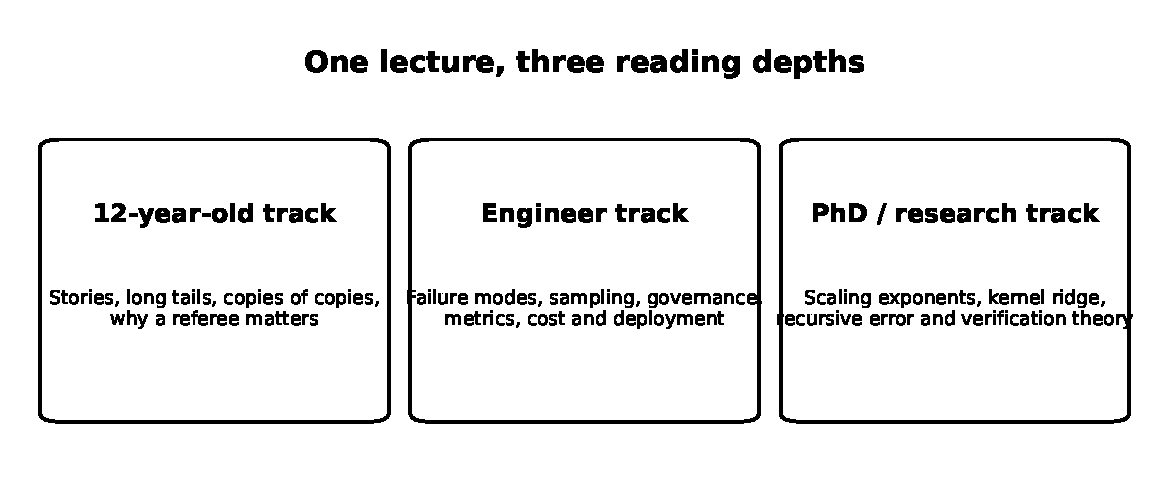
\includegraphics[width=0.95\textwidth]{figures/audience_ladder.pdf}
\caption{Three reading depths used in this document.}
\label{fig:audience}
\end{figure}

The following audience map is therefore appropriate.

\begin{longtable}{p{0.20\textwidth}p{0.35\textwidth}p{0.35\textwidth}}
\toprule
\textbf{Reader} & \textbf{What can be understood directly} & \textbf{What requires additional background} \\
\midrule
Twelve-year-old & Copies of copies lose unusual details; a referee can keep only correct attempts; more examples are not always more knowledge. & Probability laws, asymptotics, ridge regression, autoregressive likelihoods. \\
Engineer & Tail coverage, pseudo-label drift, sampling controls, verification economics, evidence lineage, deployment risks. & Formal scaling exponents, kernel spectra, high-dimensional limits. \\
Graduate / PhD & Derivations, asymptotic regimes, recursive error terms, verifier phase transitions, modified scaling laws. & Full proofs and extensions beyond the paper assumptions. \\
Research programme owner & How to turn these results into hypotheses, metrics, benchmarks, governance and architecture. & Empirical validation on the target system. \\
\bottomrule
\end{longtable}

\subsection{What this document is and is not}

This report is four things at once:

\begin{enumerate}[leftmargin=*]
  \item a pedagogical guide to the lecture;
  \item a technical synthesis of the associated papers;
  \item a critical orientation for \MMALS, \STRATQ, probabilistic MTP, and Test Data Governance;
  \item a reproducible experimental roadmap.
\end{enumerate}

It is not:

\begin{itemize}[leftmargin=*]
  \item a verbatim transcript;
  \item a claim that every practical synthetic-data pipeline collapses;
  \item a proof that MMALS already exhibits or avoids the proposed phenomena;
  \item an official biography or exhaustive map of Julia Kempe's collaborators;
  \item a replacement for reading the original papers.
\end{itemize}

\begin{cautionbox}
Several conclusions in this report are research hypotheses for MMALS and STRAT-Q. They are deliberately marked as orientations rather than validated results. The correct next step is controlled experimentation, not architectural overclaiming.
\end{cautionbox}

\section{The twelve-year-old chapter: the library of copies}

Imagine a giant library. The library contains common books, rare books, notebooks, maps, strange dictionaries, and a few very important emergency manuals.

A robot reads the library and learns to write new books. Most of its books look good. The robot especially likes common stories because it has seen them many times. It is less good at rare books because it has seen them only once or twice.

Now imagine that a second robot is trained mostly on books written by the first robot.

\subsection{The first problem: rare books disappear}

The first robot writes many common stories and very few rare ones. The second robot therefore sees even fewer rare stories. A third robot sees almost none.

After several generations, the library may still be very large, but it has become less varied.

\begin{keyidea}
A bigger pile of books is not necessarily a richer library.
\end{keyidea}

This is the idea of a \emph{long tail}. A small number of things are very common, while a huge number of things are rare. The rare things may include unusual words, difficult mathematical cases, rare machine failures, or a route that only one MMALS host knows how to solve.

\subsection{The second problem: a wrong answer becomes a schoolbook answer}

Suppose a teacher makes a small mistake in a geometry exercise. A student copies the answer. The next year's teacher uses the student's notebook as the official solution. The mistake is now no longer seen as a mistake: it has become the new lesson.

That is what can happen with synthetic labels. The input question may still be real, but the answer used for training comes from an older model.

\subsection{The third problem: being consistent is not the same as being correct}

A robot can become extremely good at copying another robot's style. It may produce very consistent answers. But if the first robot was wrong, the new robot can be precisely wrong.

This is similar to a ruler that is two millimetres too short. Measuring the same object one thousand times gives a very precise answer, but the answer remains biased.

\subsection{How a verifier helps}

Now add a referee who can check each answer.

The robot writes one hundred possible answers. Perhaps only twenty are correct. The referee keeps the correct ones and throws away the others. The next robot trains on the selected answers.

The first robot did not need to be perfect. It only needed to produce enough good candidates, and the referee needed to recognize them.

\[
\text{many attempts} + \text{reliable checking} \longrightarrow \text{better training data}.
\]

A calculator can verify arithmetic. A compiler can verify whether code is valid. A physical simulator can check whether a proposed design respects constraints. A human expert can verify a difficult business claim.

\subsection{The MMALS forest}

Think of MMALS as a forest with different host trees. The mycelial network carries information between them. One tree is good at common tasks. Another tree is useful for rare geometric tasks. A third tree helps when memory is needed.

If the forest only replays the routes used by the common tree, the rare trees receive no work. They stop improving and may become useless. The forest looks simpler and calmer, but it has lost abilities.

A healthy forest does not activate every tree for every problem. That would waste energy. It does keep the rare trees alive when they provide a real function.

\begin{mmalsnote}
The goal is not maximum diversity at every moment. The goal is to use a simple route for a simple problem while preserving the ability to form a more complex route when the problem changes.
\end{mmalsnote}

\subsection{The test-data lesson}

Imagine testing a bicycle only on a smooth road. You can repeat the test one million times. You will know the smooth-road behaviour very well. You still know almost nothing about ice, mud, broken pavement, or a steep descent.

Synthetic testing is useful when it creates valid versions of those rare roads. It is misleading when it produces one million slightly different smooth roads and calls that complete coverage.

\subsection{The whole story in six sentences}

\begin{enumerate}[leftmargin=*]
  \item Real data contain common cases and rare cases.
  \item Generators often reproduce common cases more easily.
  \item Copies of copies can lose rare cases and repeat old errors.
  \item More copied data can improve repetition without adding new knowledge.
  \item Real anchors and independent verifiers can correct the loop.
  \item A good learning system must remain able to be surprised.
\end{enumerate}

\section{The engineer chapter: distributions, failure modes, and controls}

\subsection{Scaling laws are resource-balance laws}

A standard empirical scaling model decomposes the test loss into terms associated with limited data and limited model capacity:
\[
E(T,d) \approx \left(\frac{T_c}{T}\right)^a + \left(\frac{d_c}{d}\right)^b.
\]
The equation should be read like a bottleneck model. Increasing $d$ cannot compensate indefinitely for inadequate $T$, and increasing $T$ cannot compensate indefinitely for inadequate $d$. For engineering, the important point is not the exact exponent but the structure: every improvement programme eventually becomes limited by the resource that is no longer growing appropriately \citep{kaplan2020scaling,hoffmann2022chinchilla}.

Synthetic data changes this picture because it changes what $T$ means. Ten million examples generated by the same teacher are not equivalent to ten million independent observations. We therefore distinguish:
\[
T_{\mathrm{raw}} \neq T_{\mathrm{effective}}.
\]
A useful conceptual decomposition is
\[
T_{\mathrm{effective}}
= T_{\mathrm{raw}}
\times q_{\mathrm{quality}}
\times q_{\mathrm{diversity}}
\times q_{\mathrm{independence}}
\times q_{\mathrm{freshness}}
\times q_{\mathrm{verification}}.
\]
This is not a universal statistical estimator. It is an engineering reminder that volume must be discounted when examples are correlated, stale, weakly verified, or narrow in support.

\subsection{Emergence: transition, threshold, or metric artefact?}

The literature on emergent abilities reports tasks that remain near random performance for smaller models and then improve sharply at larger scale \citep{wei2022emergent}. Engineers should separate three mechanisms:

\begin{enumerate}[leftmargin=*]
  \item \textbf{Internal transition.} The model discovers a reusable representation or composition.
  \item \textbf{Exposure threshold.} Rare but necessary examples finally become numerous enough.
  \item \textbf{Metric threshold.} A continuous internal improvement is converted into a discontinuous score such as exact match \citep{schaeffer2023mirage}.
\end{enumerate}

A system claim should therefore include both final metrics and continuous precursors: loss, margin, calibration, edit distance, residual reduction, partial correctness, and causal contribution of components.

\subsection{Zipf distributions and the long tail}

A ranked frequency distribution often follows
\[
p(i) = C i^{-\beta}, \qquad \beta>1.
\]
A small number of events dominate the mass, while many events are individually rare. In language, these can be rare words or constructions. In software engineering, they can be unusual dependency combinations, specific deployment states, rare load spikes, or uncommon failure sequences.

Uniform input sampling does not imply uniform output sampling. In the GCD example, uniformly sampled integer pairs induce approximately
\[
\Prob(\gcd(a,b)=k) \propto k^{-2}.
\]
Consequently, a model sees many examples with small GCDs and very few with large or structurally rare GCDs. Training distributions determine which arithmetic skills are learned and when \citep{charton2024gcd}.

\subsection{Perplexity is model-relative surprise}

For a token sequence $X=(x_1,\ldots,x_L)$, perplexity is
\[
\mathrm{PPL}(X)
= \exp\left(
-\frac{1}{L}\sum_{t=1}^{L}
\log p_\theta(x_t\mid x_{<t})
\right).
\]
Low perplexity indicates that the model assigned high probability to the observed continuation. High perplexity indicates surprise. It does not directly distinguish:

\begin{itemize}[leftmargin=*]
  \item useful novelty;
  \item domain-specific content;
  \item corrupted text;
  \item tokenization artefacts;
  \item missing context;
  \item genuine complexity.
\end{itemize}

Therefore, perplexity is a useful triage signal, not a quality certificate. It should be combined with data quality, semantic validity, novelty, and task relevance.

\subsection{The Hutter memory baseline}

The infinite-memory model intentionally removes generalization. Each input $i$ has a deterministic correct label $j_i$. The learner answers correctly only if the pair has appeared in the training set:
\[
\widehat f(i)=
\begin{cases}
 j_i, & \text{if }(i,j_i)\in D_T,\\
 \perp, & \text{otherwise.}
\end{cases}
\]
The test error is the probability mass of unseen events:
\[
E_T = \sum_{i\ge 1}p(i)(1-p(i))^T.
\]
For $p(i)\propto i^{-\beta}$,
\[
E_T \asymp T^{-(1-1/\beta)}.
\]
This is a scaling law produced by memorization and a heavy-tailed distribution \citep{hutter2021learning}. It is an essential baseline because it prevents a misleading interpretation:

\begin{keyidea}
A power-law improvement curve is evidence of increasing coverage. It is not, by itself, evidence of abstraction, reasoning, compositionality, or self-organization.
\end{keyidea}

For MMALS, the corresponding baseline is an exact context-to-route memory. Any claimed geometric or collaborative intelligence must outperform this baseline on unseen variants and novel compositions.

\subsection{Three ways to damage a tail}

\paragraph{Top-$p$ truncation.} Nucleus sampling keeps the smallest set of outcomes whose cumulative probability exceeds $p_0$. Everything outside the set receives probability zero. A small discarded probability mass can contain a very large number of rare possibilities.

\paragraph{Temperature narrowing.} If
\[
q_i^{(\tau)} \propto p_i^{1/\tau},
\]
then for a power law $p_i\propto i^{-\beta}$,
\[
q_i^{(\tau)} \propto i^{-\beta/\tau}.
\]
For $\tau<1$, the exponent increases and rare events become even rarer.

\paragraph{Finite sampling.} An event with probability $p_i$ is absent from a sample of size $N$ with probability
\[
(1-p_i)^N \approx e^{-Np_i}.
\]
Even a perfectly calibrated generator loses sufficiently rare events in a finite synthetic corpus.

These mechanisms differ operationally, but all reduce the coverage available to the next learner.

\subsection{Cut tails create a hard error floor}

If synthetic data omit all ranks above $k$, the modified Hutter scaling law is
\[
E_{\mathrm{test}}
\asymp T^{-(\beta-1)/\beta}
+ k^{-(\beta-1)}.
\]
The first term is ordinary finite-data error. The second is the missing probability mass beyond the cutoff. The second term does not decrease with $T$ \citep{dohmatob2024tails}.

\begin{figure}[H]
\centering
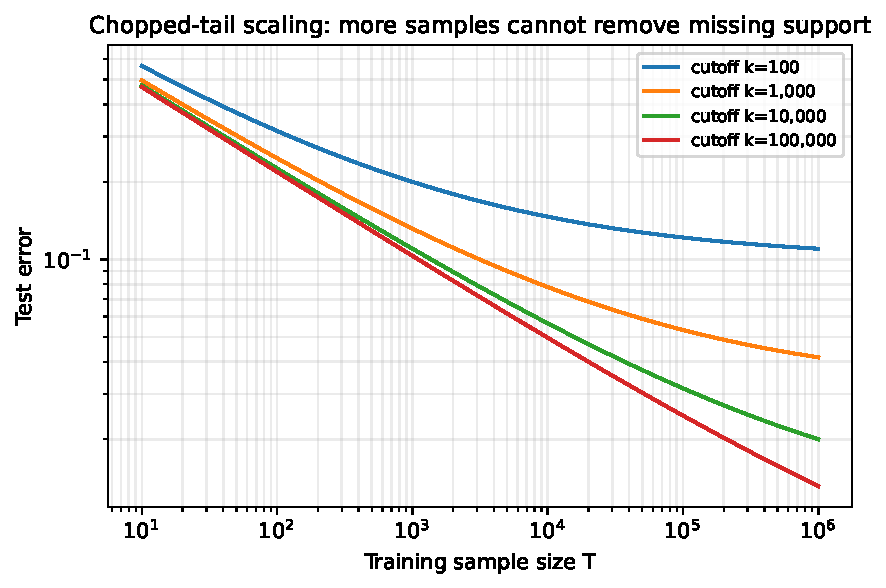
\includegraphics[width=0.86\textwidth]{figures/chopped_tail_scaling.pdf}
\caption{Original reconstruction of the chopped-tail scaling law. Each curve initially improves with sample size and then approaches a cutoff-dependent floor.}
\label{fig:chopped}
\end{figure}

The crossover occurs near
\[
T^\star \asymp k^\beta.
\]
Before $T^\star$, more samples help. After $T^\star$, the system is support-limited. The engineering action must change from ``generate more'' to ``restore missing regimes.''

\subsection{Recursive relabeling: same inputs, drifting truth}

Tail loss is not the only failure mode. The input distribution can remain unchanged while the labels become synthetic. In linear form,
\[
x\sim\mathcal N(0,\Sigma),\qquad
 y=x^\top w_0+\epsilon.
\]
A first ridge model estimates $\widehat w_1$, generates new labels, and a second model estimates $\widehat w_2$. The chain is
\[
P_{\Sigma,w_0,\sigma_0^2}
\rightarrow P_{\Sigma,\widehat w_1,\sigma_1^2}
\rightarrow P_{\Sigma,\widehat w_2,\sigma_2^2}
\rightarrow \cdots.
\]
Each generation can inherit previous bias and add new variance. More examples allow a student to fit the synthetic teacher more accurately, but do not automatically recover $w_0$ \citep{dohmatob2024regression}.

\begin{figure}[H]
\centering
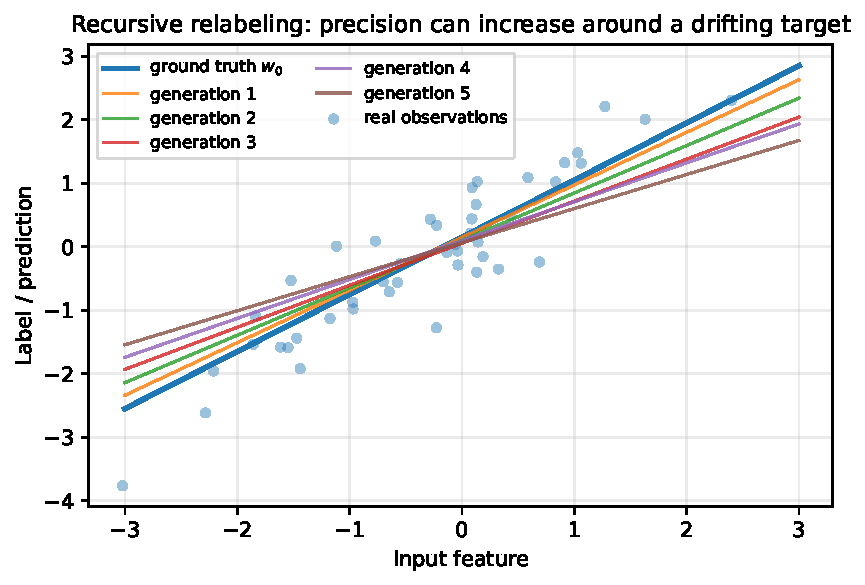
\includegraphics[width=0.82\textwidth]{figures/recursive_relabeling.pdf}
\caption{Conceptual recursive relabeling. Later generations may become precise around a drifting target.}
\label{fig:recursive}
\end{figure}

The practical analogy is instrument calibration. Repeatedly calibrating instrument $g+1$ against instrument $g$, rather than against the physical reference, can create a stable but biased chain.

\subsection{Model collapse is conditional, not mystical}

The broad literature shows different outcomes because the protocols differ. Collapse is more likely when:

\begin{itemize}[leftmargin=*]
  \item each generation replaces the original data;
  \item pseudo-label errors are treated as ground truth;
  \item sampling removes tails;
  \item model approximation errors are correlated across generations;
  \item the next learner has no independent corrective signal.
\end{itemize}

Stability is more plausible when:

\begin{itemize}[leftmargin=*]
  \item real data are retained or accumulated;
  \item fresh real observations continue to arrive;
  \item generated candidates are independently verified;
  \item the synthetic source targets under-covered regimes rather than only common ones;
  \item the mixture and regularization are adapted to lineage and uncertainty.
\end{itemize}

This reconciles apparently conflicting results such as recursive degradation \citep{shumailov2024curse,alemohammad2024mad} and stability under accumulation or controlled mixing \citep{bertrand2024stability,gerstgrasser2024inevitable}.

\subsection{When synthetic data help}

Let
\[
T=T_{\Real}+T_{\AI}.
\]
When real data are scarce relative to the preserved support, synthetic data can reduce finite-sample error:
\[
E_{\mathrm{test}}
\asymp (T_{\Real}+T_{\AI})^{-(1-1/\beta)}
+ k^{-(\beta-1)}.
\]
They densify the known support. They do not automatically extend it.

\begin{figure}[H]
\centering
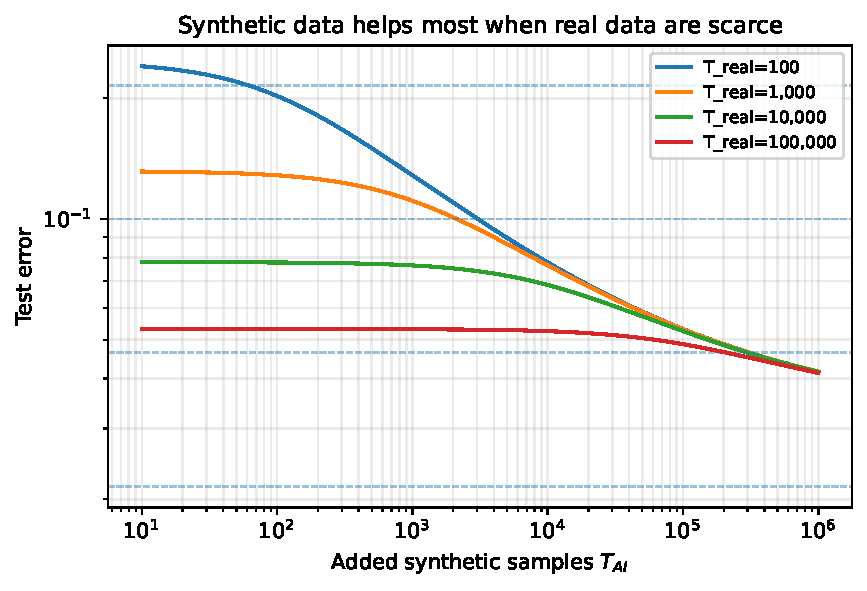
\includegraphics[width=0.86\textwidth]{figures/real_synthetic_mix.pdf}
\caption{Synthetic samples are most useful when the real sample is small. Benefits saturate at a support-dependent floor.}
\label{fig:mix}
\end{figure}

This creates four distinct business cases:

\begin{longtable}{p{0.20\textwidth}p{0.35\textwidth}p{0.35\textwidth}}
\toprule
\textbf{Use} & \textbf{Potential value} & \textbf{Main risk} \\
\midrule
Augmentation & More variation around known cases & Repetition disguised as diversity \\
Distillation & Transfer from a stronger model & Student inherits teacher's support ceiling \\
Rare-event generation & Increased exposure to selected regimes & Invalid or unrepresentative scenarios \\
Recursive self-training & Low-cost scale & Error and tail accumulation \\
\bottomrule
\end{longtable}

\subsection{Verification changes the economics}

The most constructive result is that an imperfect generator can be useful if good candidates can be recognized more cheaply than they can be generated directly \citep{feng2025verification}. The pipeline is:
\[
\text{seed data}
\rightarrow \text{generator}
\rightarrow \text{many candidates}
\rightarrow \text{verifier}
\rightarrow \text{filtered retraining set}.
\]

\begin{figure}[H]
\centering
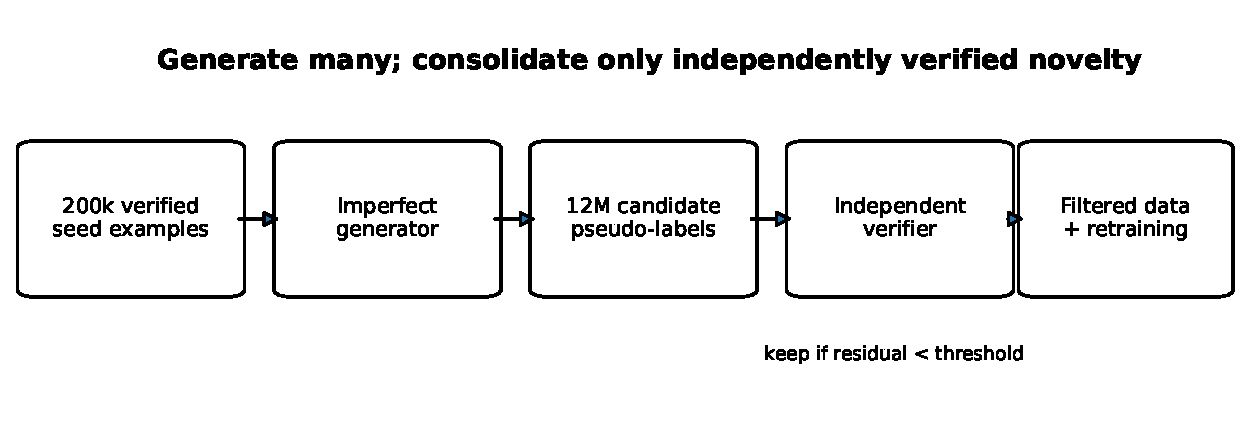
\includegraphics[width=0.96\textwidth]{figures/verification_bootstrap.pdf}
\caption{Verifier-based synthetic-data bootstrapping.}
\label{fig:verification}
\end{figure}

Let
\[
\phi = \Prob(\text{kept}\mid\text{correct}),\qquad
\psi = \Prob(\text{kept}\mid\text{incorrect}).
\]
A useful verifier has high $\phi$ and low $\psi$. Perfection is unnecessary; enrichment is necessary. The resulting system must still account for verification bias: a verifier that accepts only easy or conventional cases can create a new tail problem.

\subsection{Engineer checklist}

Before using synthetic data for training or testing, ask:

\begin{enumerate}[leftmargin=*]
  \item What independent information does the generator add?
  \item Which parts of the target distribution are absent or underrepresented?
  \item What are the sampling parameters and generation depth?
  \item Who or what provides the oracle?
  \item Is verification cheaper than direct production of correct labels?
  \item Are real anchors preserved and refreshed?
  \item Is success measured on a real, independent, uncontaminated evaluation set?
  \item Are average performance and rare-regime performance both reported?
  \item Can the system detect that more data no longer reduce the relevant uncertainty?
\end{enumerate}

\section{The PhD chapter: formal models and asymptotic mechanisms}

\subsection{From empirical scaling to distribution-sensitive scaling}

Empirical neural scaling laws often take the form
\[
\mathcal L(N,D,C)
\approx \mathcal L_\infty
+ a_N N^{-\alpha}
+ a_D D^{-\delta}
+ a_C C^{-\gamma},
\]
where $N$ denotes parameters, $D$ data, and $C$ compute. The lecture's central move is to treat the training distribution as an evolving object rather than a fixed background assumption. Let $P_0$ be the natural or human distribution and $P_g$ the distribution available at generation $g$. The learner is then a map
\[
\mathcal A:(P_g,T_g,\mathcal M_g)\mapsto f_g,
\]
and the generator induces a second map
\[
\mathcal G:f_g\mapsto P_{g+1}.
\]
Recursive training studies the composite dynamical system
\[
P_{g+1}=\mathcal G(\mathcal A(P_g,T_g,\mathcal M_g)).
\]
Model collapse is therefore not a single scalar event. It can mean contraction of support, altered tail exponent, increasing bias, increasing variance, worsening calibration, loss of skills, or a changed scaling exponent.

\subsection{The infinite-memory model}

Let inputs $i\in\mathbb N$ follow
\[
p_i = \frac{i^{-\beta}}{\zeta(\beta)},\qquad \beta>1,
\]
and let labels be deterministic, $y_i=f^\star(i)$. Given $T$ iid samples, the infinite-memory predictor answers correctly if $i$ was observed. Its error is
\[
E_T = \sum_{i=1}^{\infty} p_i(1-p_i)^T.
\]
For small $p_i$,
\[
(1-p_i)^T \approx e^{-Tp_i},
\]
so
\[
E_T \approx \sum_i p_i e^{-Tp_i}.
\]
A threshold analysis sets $Tp_{i^\star}\approx 1$, giving
\[
i^\star \asymp T^{1/\beta}.
\]
The remaining tail mass is
\[
\sum_{i>i^\star} i^{-\beta}
\asymp \int_{i^\star}^{\infty}x^{-\beta}\,dx
\asymp (i^\star)^{1-\beta},
\]
and therefore
\[
E_T\asymp T^{-(\beta-1)/\beta}.
\]
The exponent
\[
c=1-\frac{1}{\beta}
\]
is determined by the tail. The mechanism is occupancy, not rule learning.

\subsection{Chopped tails}

Define a synthetic distribution $Q_k$ with support restricted to $i\le k$. Evaluation remains under $P_0$. The error separates into an in-support occupancy term and missing tail mass:
\[
E_{T,k}
= \sum_{i\le k}p_i\Prob(i\text{ unseen})
+ \sum_{i>k}p_i.
\]
Under the same asymptotic approximations,
\[
E_{T,k}
\asymp T^{-(\beta-1)/\beta}
+ k^{-(\beta-1)}.
\]
Equivalently, up to constants,
\[
E_{T,k}
\asymp \min(T,k^\beta)^{-(\beta-1)/\beta}.
\]
The crossover $T\asymp k^\beta$ separates sample-limited and support-limited regimes. This structure is more informative than the generic statement ``synthetic data are worse'' because it identifies the intervention required in each regime.

\subsection{Narrowed tails}

Suppose the synthetic distribution preserves support but changes the exponent from $\beta$ to $\beta'>\beta$. This is a narrower tail. The learner is now exposed to rare events at a rate governed by $\beta'$, while evaluation may remain governed by $\beta$. Depending on the precise model, one obtains altered learning exponents and crossover behaviour rather than an immediate hard floor \citep{dohmatob2024tails}.

Temperature transformation illustrates the mechanism. If $p_i\propto i^{-\beta}$ and
\[
q_i^{(\tau)}\propto p_i^{1/\tau},
\]
then
\[
q_i^{(\tau)}\propto i^{-\beta/\tau}.
\]
For $\tau<1$, $\beta/\tau>\beta$ and the tail is narrowed. Top-$p$ sampling can instead induce an explicit cutoff.

\subsection{Multiple generations}

Let each generation use $T_0$ samples from the preceding synthetic distribution and let the final model use $T$ samples from generation $n$. In the simplified tail model, each arrow introduces another scaling term. A representative expression is
\[
E_{\mathrm{test}}^{(n)}(T)
\asymp T^{-c} + C_n T_0^{-c},
\]
with $C_n$ often growing with $n$. If $T_0\asymp T$, then
\[
E_{\mathrm{test}}^{(n)}(T)\lesssim nT^{-c}
\]
in the corresponding regime. This is not a universal exact law for LLMs; it is a structural warning that each recursive stage can contribute an additional irreducible approximation or sampling term.

For an autoregressive model,
\[
q_g(y\mid x)
=\prod_{t=1}^{L}q_g(y_t\mid x,y_{<t}).
\]
An early generated token changes the conditioning history for all later tokens. Recursive generation therefore transforms both local token probabilities and trajectory distributions.

\subsection{Mixing real and synthetic data}

Let
\[
T=T_{\Real}+T_{\AI},\qquad
\pi=\frac{T_{\Real}}{T}.
\]
In the simplified chopped-tail setting, when $T_{\Real}\ll k^\beta$,
\[
E_{\mathrm{test}}
\asymp (T_{\Real}+T_{\AI})^{-(1-1/\beta)}
+ k^{-(\beta-1)}.
\]
Synthetic data reduce occupancy error but not the missing-support term. Once sufficiently rich real data become available, the asymptotic behaviour can return to
\[
E_{\mathrm{test}}
\asymp T_{\Real}^{-(1-1/\beta)}.
\]
This motivates the interpretation of synthetic data as a bootstrap under scarcity rather than a guaranteed asymptotic replacement for real data.

\subsection{Grokking under mixed data}

Suppose synthetic examples encode an easier but biased rule and real examples encode a more general rule. Optimisation can first fit the high-density synthetic structure and only later discover the real rule. The observed curve may show:
\[
\text{rapid train fit}
\rightarrow \text{validation plateau}
\rightarrow \text{late transition}.
\]
This resembles grokking \citep{power2022grokking}. The engineering consequence is that early stopping based on a single aggregate validation metric can terminate before the transition. The research consequence is that late improvement must not be asserted as proof of a specific internal mechanism without representation-level and causal evidence.

\subsection{Kernel ridge regression}

Consider Gaussian design
\[
x\sim\mathcal N(0,\Sigma),
\qquad y=x^\top w_0+\epsilon,
\qquad \epsilon\sim\mathcal N(0,\sigma_0^2).
\]
At generation $g$, ridge regression estimates
\[
\widehat w_g
=\arg\min_w
\frac{1}{T_g}\|y_g-X_gw\|_2^2
+\lambda_g\|w\|_2^2.
\]
The closed form is
\[
\widehat w_g
=\left(X_g^\top X_g+T_g\lambda_g I\right)^{-1}X_g^\top y_g.
\]
Synthetic relabeling defines
\[
y_{g+1}=X_{g+1}\widehat w_g+\epsilon_{g+1}.
\]
Writing $e_g=\widehat w_g-w_0$ yields a recursion of the schematic form
\[
e_g=A_ge_{g-1}+b_g+\xi_g,
\]
where $A_g$ propagates inherited error, $b_g$ captures systematic regularization bias, and $\xi_g$ captures new sample and label noise. The resulting risk has contributions from clean-data estimation, inherited synthetic bias, and generation-specific variance \citep{dohmatob2024regression}.

The ridge parameter creates a bias--variance trade-off. Small $\lambda$ fits synthetic noise and teacher error; large $\lambda$ shrinks the target excessively. Hence an optimal $\lambda_g^\star$ can depend on generation depth and synthetic noise. Adaptive regularization mitigates some regimes but cannot create information absent from the labels.

\subsection{Strong model collapse}

The later strong-collapse result shows that, in a supervised regression setting, even a small constant synthetic fraction can alter asymptotic behaviour, so that increasing dataset size does not recover the clean scaling law \citep{dohmatob2025strong}. The practical lesson is not that every $1\%$ synthetic mixture is disastrous. It is that a constant synthetic fraction is not asymptotically negligible merely because it is numerically small. Its effect depends on dependence structure, model class, label bias, and scaling regime.

\subsection{Verifier-based selection}

Let a generator produce candidate pairs $(x,\widetilde y)$, with latent correctness $C\in\{0,1\}$. A verifier produces acceptance $A\in\{0,1\}$. Define
\[
\phi=\Prob(A=1\mid C=1),
\qquad
\psi=\Prob(A=1\mid C=0).
\]
The accepted-set correctness is
\[
\Prob(C=1\mid A=1)
=\frac{\phi\Prob(C=1)}{
\phi\Prob(C=1)+\psi\Prob(C=0)}.
\]
Verification is useful when it sufficiently enriches correctness and does not destroy the relevant support. The verifier can be imperfect, but its selective advantage must be measurable \citep{feng2025verification}.

There are two distinct risks:

\begin{enumerate}[leftmargin=*]
  \item \textbf{False acceptance:} bad examples enter the training set.
  \item \textbf{Selection bias:} valid but unusual examples are systematically rejected.
\end{enumerate}

A verifier can therefore prevent label collapse while creating tail collapse. Both precision and support preservation must be evaluated.

\subsection{A general decomposition for recursive synthetic learning}

A useful research abstraction is
\[
\begin{aligned}
E_g ={}& E_{\mathrm{clean}}(T_g,N_g)
+E_{\mathrm{support}}(P_0,P_g)
+E_{\mathrm{label}}(f_{g-1},f^\star)\\
&+E_{\mathrm{dependence}}(D_g)
+E_{\mathrm{verification}}(V_g)
+E_{\mathrm{shift}}(P_g,P_{\mathrm{deploy}}).
\end{aligned}
\]
Each term suggests a different intervention:

\begin{longtable}{p{0.25\textwidth}p{0.30\textwidth}p{0.35\textwidth}}
\toprule
\textbf{Error term} & \textbf{Diagnosis} & \textbf{Intervention} \\
\midrule
Clean estimation & Insufficient samples or capacity & More data, capacity, compute, better optimisation \\
Support & Missing or narrowed regimes & Real anchors, targeted simulation, diversified generation \\
Label & Biased pseudo-oracle & Independent verification, relabeling, uncertainty weighting \\
Dependence & Duplicates and correlated ancestry & Lineage-aware effective sample size \\
Verification & Weak or biased filter & Calibrate verifier, stratify acceptance, preserve tails \\
Shift & Training/deployment mismatch & Fresh data, monitoring, recalibration \\
\bottomrule
\end{longtable}

\begin{keyidea}
The phrase ``model collapse'' should be replaced, whenever possible, by a specific diagnosis: support contraction, recursive label bias, dependence inflation, verifier selection bias, or deployment shift.
\end{keyidea}

\section{Julia Kempe and the collaboration environment}

\subsection{Positioning of the speaker}

As of June 2026, Julia Kempe's official academic page describes her as a researcher in the foundations of AI and machine learning, a Silver Professor at NYU's Courant Institute and Center for Data Science, currently on leave, and a Director and Senior Researcher at Meta FAIR, where she leads the Foundations of Reasoning Team (FoRT) \citep{kempebio2026,kempecv2026}. Her trajectory combines mathematics, theoretical computer science, quantum information, machine learning theory, data science leadership, and industrial research.

This matters for interpreting the lecture. The presentation is not a general advocacy talk about synthetic data. It is characteristic of a research environment that seeks mathematically tractable models, then validates them on controlled transformer and LLM experiments. The approach moves repeatedly between:

\begin{itemize}[leftmargin=*]
  \item asymptotic theory;
  \item simplified models that isolate one mechanism;
  \item algorithmic tasks with exact or interpretable structure;
  \item larger text-generation experiments;
  \item implications for data curation and future model training.
\end{itemize}

\subsection{Selected synthetic-data collaboration network}

The papers most directly connected to the lecture involve a recurring group of collaborators:

\begin{itemize}[leftmargin=*]
  \item Elvis Dohmatob;
  \item Yunzhen Feng;
  \item Pu Yang;
  \item Francois Charton;
  \item Arjun Subramonian;
  \item Julia Kempe.
\end{itemize}

The collaborations connect Meta FAIR, NYU's Center for Data Science and Courant Institute, and, in the verifier paper, Peking University \citep{dohmatob2024tails,dohmatob2024regression,feng2025verification,dohmatob2025strong}. The lecture itself belongs to the IHES/CNRS mathematics-and-LLM ecosystem \citep{ihesmathllm2024}.

\begin{figure}[H]
\centering
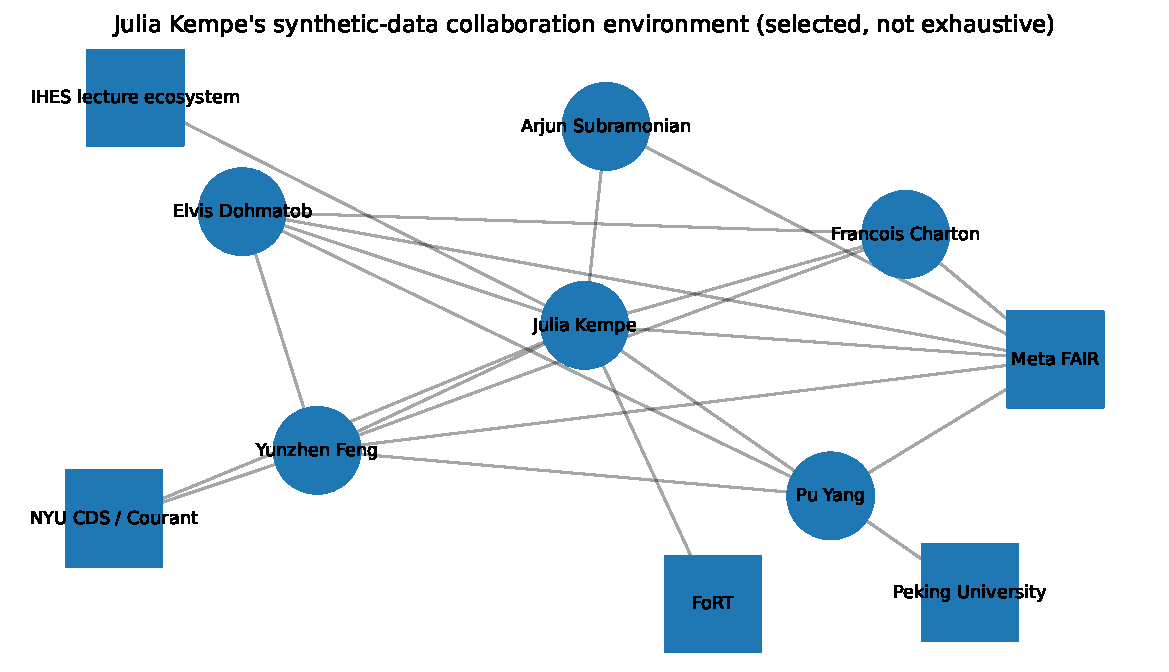
\includegraphics[width=0.96\textwidth]{figures/julia_collaboration_network.pdf}
\caption{Selected collaboration environment reconstructed from the cited synthetic-data papers and current institutional roles. It is intentionally not exhaustive.}
\label{fig:julia-network}
\end{figure}

\subsection{Why the team structure is scientifically relevant}

The research programme benefits from several complementary competencies.

\begin{longtable}{p{0.25\textwidth}p{0.30\textwidth}p{0.35\textwidth}}
\toprule
\textbf{Competence} & \textbf{Role in the programme} & \textbf{Visible contribution in the lecture line} \\
\midrule
Learning theory & Formalize generalization and asymptotics & Modified scaling laws and strong-collapse regimes \\
High-dimensional statistics & Separate bias, variance, spectrum and regularization & Kernel/ridge analysis \\
Interpretable mathematical tasks & Provide exact structure and controllable distributions & GCD and eigenvalue experiments \\
Large-model experimentation & Test whether toy-model mechanisms survive in LLM settings & Llama-based text-generation experiments \\
Verification theory & Characterize when filtering synthetic candidates helps & Verifier true/false acceptance analysis \\
Data-centric AI & Treat the corpus as a designed object rather than passive input & Tail preservation and collapse-aware curation \\
\bottomrule
\end{longtable}

The environment is therefore neither purely theoretical nor purely empirical. It resembles a loop:
\[
\text{mechanism hypothesis}
\rightarrow \text{tractable theorem}
\rightarrow \text{controlled experiment}
\rightarrow \text{larger-model test}
\rightarrow \text{new mechanism}.
\]

\subsection{A broader reasoning-and-mathematics context}

Kempe's current official role at Meta FAIR places the work in a broader Foundations of Reasoning environment. That environment is relevant to MMALS because it studies not only output quality but also the conditions under which reasoning, mathematical structure, verification, and data generation can scale. The synthetic-data papers should thus be read as part of a wider question:

\begin{quote}
How can a model generate, select, preserve, and improve structured knowledge without turning its previous approximations into an unquestioned source of truth?
\end{quote}

That question is directly aligned with MMALS memory consolidation, protocol verification, route selection, and functional specialization.

\subsection{Critical reading of authority}

The speaker's credentials and institutional environment justify taking the work seriously. They do not remove the need for critical evaluation. The models are deliberately simplified, practical pipelines vary, and later literature has shown that replacement, accumulation, verification, and mixture policies can lead to different outcomes.

The correct use of this research is therefore:

\begin{enumerate}[leftmargin=*]
  \item preserve the precise assumptions of each theorem;
  \item reproduce the controlled experiments;
  \item test whether the mechanism transfers to the target architecture;
  \item avoid using the prestige of the environment as a substitute for evidence.
\end{enumerate}

\section{Research orientation for MMALS}

\subsection{Why synthetic-data collapse maps naturally to MMALS}

MMALS does not only process external datasets. It also produces internal artefacts:
\[
\text{context}
\rightarrow
\text{host activations}
\rightarrow
\text{route}
\rightarrow
\text{memory trace}
\rightarrow
\text{future routing evidence}.
\]
If these artefacts are replayed, summarized, or used as pseudo-labels for later versions, MMALS becomes a recursive data-generation system. The analogue of a token distribution is a distribution over functional regimes, hosts, routes, memories, and collaborative trajectories.

Let $r\in\mathcal R$ denote a route and let
\[
p_g(r\mid x,m,z)
\]
be the routing distribution at generation or learning cycle $g$. A self-reinforcing loop can occur:
\[
p_g(r)
\rightarrow
D_g^{\mathrm{trace}}
\rightarrow
\text{router update}
\rightarrow
p_{g+1}(r).
\]
A route that is slightly more frequent receives more replay, more gradient, and more memory support. This can increase its probability even when its original advantage was accidental.

\subsection{Functional model collapse}

We define \emph{functional model collapse} as a reduction in the effective set of accessible, causally useful behaviours while average performance or route stability may remain high.

A practical definition requires four elements:

\begin{enumerate}[leftmargin=*]
  \item a target distribution of functional regimes $P_{\mathrm{target}}$;
  \item a set of accessible routes $\mathcal R_g$;
  \item a causal utility test $U(r)$;
  \item a comparison across learning cycles or generations.
\end{enumerate}

The effective functional support can be written conceptually as
\[
K_{\mathrm{eff}}(g)
=
\sum_{r\in\mathcal R}
\ind\left[
\Prob_g(r)>\epsilon_p,
\Delta Q_r^{\mathrm{causal}}>\epsilon_q
\right].
\]
A collapse occurs when $K_{\mathrm{eff}}$ decreases materially and the missing routes correspond to real target regimes.

\begin{figure}[H]
\centering
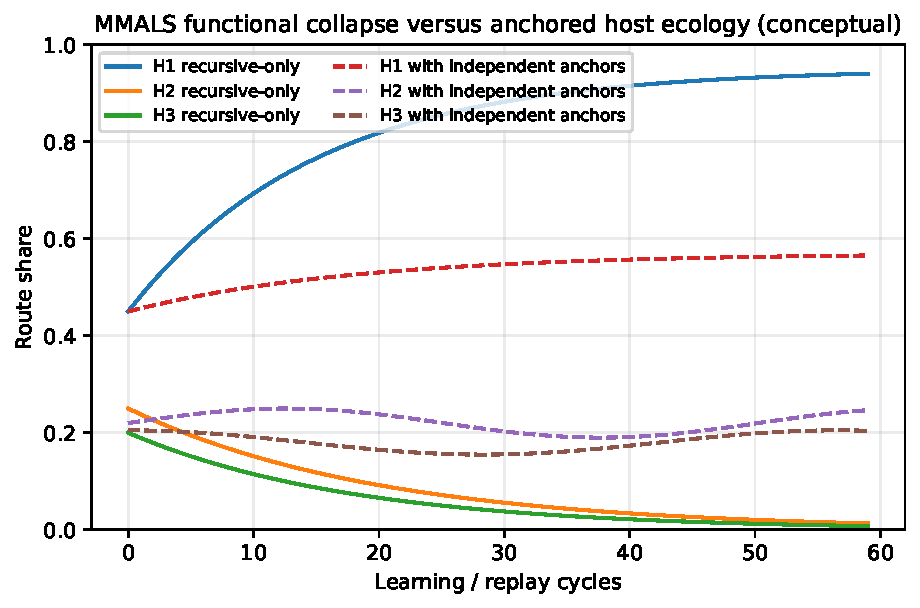
\includegraphics[width=0.90\textwidth]{figures/mmals_host_ecology.pdf}
\caption{Conceptual host ecology under recursive-only reinforcement and under continued independent anchoring. The figure is illustrative, not an empirical MMALS result.}
\label{fig:mmals-ecology}
\end{figure}

\subsection{The two collapse mechanisms in MMALS}

The two mechanisms highlighted in synthetic-data research have direct analogues.

\paragraph{Finite sampling of routes.} A useful route is rare. It is absent from replay batches, audit memory, or synthetic traces. Its hosts receive no reinforcement. Eventually the route becomes practically inaccessible.

\paragraph{Function-approximation error.} The shared latent space, energy function, or router cannot preserve all relevant regimes. Several distinct routes are smoothed into a single dominant solution.

A third MMALS-specific mechanism should be added:

\paragraph{Objective-induced collapse.} A fixed or dominant objective---for example immediate accuracy---systematically suppresses routes useful for retention, cost, stability, or future recomposition. This is especially relevant to TPUT and goal-conditioned control.

\subsection{Softmax, temperature, and route tails}

Suppose route scores are energies $E_r$ and
\[
p(r\mid x)
=\frac{\exp(-E_r/\tau)}{\sum_{r'}\exp(-E_{r'}/\tau)}.
\]
A lower temperature concentrates routing. This can be appropriate when one route is clearly superior. It is dangerous when uncertainty remains or when the concentration is reused as training truth.

The key distinction is:
\[
\text{local concentration at inference}
\neq
\text{global deletion from learning support}.
\]
MMALS should be able to use one host for a simple input while retaining other routes in the global ecology.

Hard top-$k$ or top-$p$ routing can create an exact analogue of chopped tails: routes outside the selected set receive no activity and potentially no learning signal. A softmax router with only a few parameters may therefore outperform a more elaborate hard selector if it preserves uncertainty and avoids premature support loss.

\subsection{Natural adaptability without controller proliferation}

The architectural objective established in the preceding MMALS work is not to accumulate separate boxes for routing, tail preservation, synthetic-data control, collapse prevention, novelty detection, and memory governance. Instead, a small number of local laws should generate the desired global behaviour.

Let the MMALS state be
\[
S_t=(z_t,h_t,m_t,a_t,W_t),
\]
where $z_t$ is latent context, $h_t$ host states, $m_t$ memory, $a_t$ activity allocation, and $W_t$ interaction structure. A generic dynamics is
\[
S_{t+1}
=S_t-\eta\nabla_S\mathcal E(S_t;x,g)
+\mathcal P(S_t)+\xi_t.
\]
The energy should combine task residual, cost, instability, forgetting, and unsupported redundancy:
\[
\mathcal E
=
\mathcal E_{\mathrm{task}}
+\lambda_C C
+\lambda_S \mathcal E_{\mathrm{stability}}
+\lambda_F \mathcal E_{\mathrm{forgetting}}
+\lambda_R \mathcal E_{\mathrm{redundancy}}.
\]
Synthetic lineage and verification should not necessarily become a central controller. They can become state variables that modulate local consolidation.

\subsection{Lineage-aware memory consolidation}

A memory trace can be represented as
\[
m_j=(z_j,r_j,y_j,s_j,g_j,v_j,f_j,c_j),
\]
where:

\begin{itemize}[leftmargin=*]
  \item $z_j$ is context;
  \item $r_j$ is route;
  \item $y_j$ is result;
  \item $s_j$ is source class;
  \item $g_j$ is synthetic generation depth;
  \item $v_j$ is verification strength;
  \item $f_j$ is freshness;
  \item $c_j$ is causal contribution evidence.
\end{itemize}

A conceptual consolidation law is
\[
\Delta M_j
\propto
\underbrace{\Delta Q_j^{\mathrm{verified}}}_{\text{functional gain}}
\times
\underbrace{N_j}_{\text{novelty}}
\times
\underbrace{I_j}_{\text{independence}}
\times
\underbrace{F_j}_{\text{freshness}}
\times
\underbrace{e^{-\lambda g_j}}_{\text{lineage discount}}.
\]
This expression is not proposed as a final formula. It identifies variables that should be represented explicitly and then simplified by experiment.

\begin{mmalsnote}
A trace should not become true because it is frequent. It should become influential because it remains useful under an independent residual, a causal intervention, or a verified external objective.
\end{mmalsnote}

\subsection{Reconstructive and synthetic memory}

The lecture sharpens the distinction between the two planned MMALS memory modes.

\paragraph{Reconstructive audit memory.} Stores the route, intermediate states, sources, and verification metadata required to replay or audit a decision. Its value is traceability, not compression.

\paragraph{Synthetic or compiled functional memory.} Compresses repeated successful experiences into reusable structure. Its value is low-cost transfer and abstraction.

The collapse risk is asymmetric. Reconstructive memory can become an enormous exact-match table. Synthetic memory can over-compress and remove rare distinctions. The two should constrain each other:
\[
\text{audit traces}
\leftrightarrow
\text{compiled functions}.
\]
A compiled function should remain linked to representative traces, including counterexamples and boundary cases.

\subsection{Host specialization and tail preservation}

A rare host is not automatically valuable. A dominant host is not automatically pathological. Host value should be claim-relative:
\[
V(H_i)
=\sum_r P(r)\,L(r)\,\Delta Q_{i,r}^{\mathrm{causal}}-C(H_i),
\]
where $L(r)$ is regime criticality and $C(H_i)$ the cost of maintaining or activating the host.

This leads to a better tail metric than route entropy alone. Define functional tail coverage
\[
\mathrm{FTC}
=\sum_{r\in\mathcal R_{\mathrm{tail}}}
P_{\mathrm{eval}}(r)
\ind[\Delta Q_r^{\mathrm{causal}}>0].
\]
FTC measures the probability mass of rare regimes for which MMALS retains a causally useful route.

The existing host-specialization programme should therefore combine:

\begin{itemize}[leftmargin=*]
  \item route entropy and dominance;
  \item host contribution gain;
  \item ablation impact;
  \item route swaps and candidate permutations;
  \item representation separation;
  \item route-function stability;
  \item cross-seed reproducibility;
  \item functional tail coverage;
  \item synthetic lineage depth.
\end{itemize}

\subsection{Dynamic compute as a scaling law}

MMALS should distinguish installed capacity and effective capacity:
\[
d_{\mathrm{installed}}
\quad\text{versus}\quad
 d_{\mathrm{eff}}(x)=\sum_i a_i(x)d_i.
\]
The desired property is
\[
d_{\mathrm{eff}}(x_{\mathrm{simple}})
\ll
d_{\mathrm{eff}}(x_{\mathrm{complex}}),
\]
without changing the global architecture.

A useful objective is
\[
\min_{r,a,T_{\mathrm{iter}}}
\left[
\mathcal L(x;r,a)
+\lambda_C C(r,a,T_{\mathrm{iter}})
+\lambda_F F(r)
\right].
\]
The system should spend additional computation only when it produces a measurable reduction in residual or future risk. Importantly, a difficult but invalid or corrupted input should not trigger unlimited computation. One stable state must be abstention.

\subsection{Choice of Llama or Mistral backbones}

MMALS should not be defined by a single LLM family. The scientific design should use a stable host interface:
\[
\texttt{encode},\quad
\texttt{forward},\quad
\texttt{adapt},\quad
\texttt{uncertainty},\quad
\texttt{export\_trace}.
\]

For causal host-specialization experiments, the first stage should use the same dense base backbone for all hosts, with equal parameter budgets and controlled adapters. This prevents backbone heterogeneity from masquerading as emergent specialization. A second stage should replicate the results with a different model family. A third stage may introduce heterogeneous hosts.

The selection principle is therefore:

\begin{enumerate}[leftmargin=*]
  \item choose a dense base model that fits the available hardware;
  \item avoid internal MoE routing in the first causal study;
  \item freeze exact model, tokenizer, quantization and adapter versions;
  \item use one family as the primary experiment and another as replication;
  \item compare cross-tokenizer metrics using bits-per-byte or relative deltas rather than raw perplexity alone.
\end{enumerate}

This is more durable than declaring MMALS a ``Llama architecture'' or a ``Mistral architecture.'' The backbone is a host; MMALS is the organisation of hosts.

\subsection{MMALS hypotheses generated by the lecture}

\begin{description}[leftmargin=3.2cm,style=nextline]
  \item[H1: Recursive route collapse.] Training primarily on self-generated routes reduces functional tail coverage across generations.
  \item[H2: Real-anchor recovery.] A sufficiently diverse stream of independently verified experiences restores lost route support after a delayed transition.
  \item[H3: Verification bootstrap.] Over-generating route candidates and verifying them can train a later MMALS version beyond the initial router's top-1 performance.
  \item[H4: Dynamic temperature.] State-dependent route temperature improves the cost--accuracy trade-off relative to fixed hard routing without increasing structural complexity.
  \item[H5: Dual-memory protection.] Linking compiled memories to reconstructive counterexamples reduces recursive memory collapse.
  \item[H6: Geometry-sensitive support.] A manifold-aware latent state preserves distinct functional regimes that are smoothed together in a Euclidean representation.
\end{description}

\subsection{What would count as a strong MMALS result?}

A strong result would not be ``MMALS retains high route entropy.'' It would show:

\begin{enumerate}[leftmargin=*]
  \item simple cases use short, inexpensive routes;
  \item hard cases recruit additional hosts only when they improve a verified residual;
  \item rare useful routes survive recursive replay;
  \item lost routes can be recovered by diverse real anchors;
  \item candidate verification produces a student that outperforms the teacher's top-1 routing;
  \item these effects replicate across seeds, datasets, and at least two backbone families;
  \item ablations demonstrate that memory, geometry, and collaboration are causally necessary for the claimed gains.
\end{enumerate}

\section{STRAT-Q, probabilistic MTP, and Test Data Governance}

\subsection{From data volume to evidence strength}

STRAT-Q treats a test result as evidence supporting or weakening a claim. Synthetic-data research therefore changes the semantics of a test campaign. The key variables are no longer only the number of cases and pass rate, but also:

\begin{itemize}[leftmargin=*]
  \item source and ancestry;
  \item degree of independence;
  \item freshness relative to the current product and deployment distribution;
  \item validity of the oracle;
  \item coverage of rare but decision-relevant regimes;
  \item contamination by the system under evaluation;
  \item synthetic generation depth;
  \item reviewer and consolidation status.
\end{itemize}

A conceptual evidence-strength function for evidence item $e$ and claim $c$ is
\[
S(e\mid c)
=Q_e F_e I_e V_e C_{e,c} T_{e,c},
\]
where $Q$ is quality, $F$ freshness, $I$ independence, $V$ verification, $C$ claim relevance, and $T$ tail coverage. This multiplicative form is illustrative; a production model should be probabilistically calibrated rather than assigned arbitrary scores.

\subsection{Evidence Passport}

A dataset, batch, or test result should carry an Evidence Passport. The passport extends dataset documentation and cryptographic provenance with decision semantics.

\begin{figure}[H]
\centering
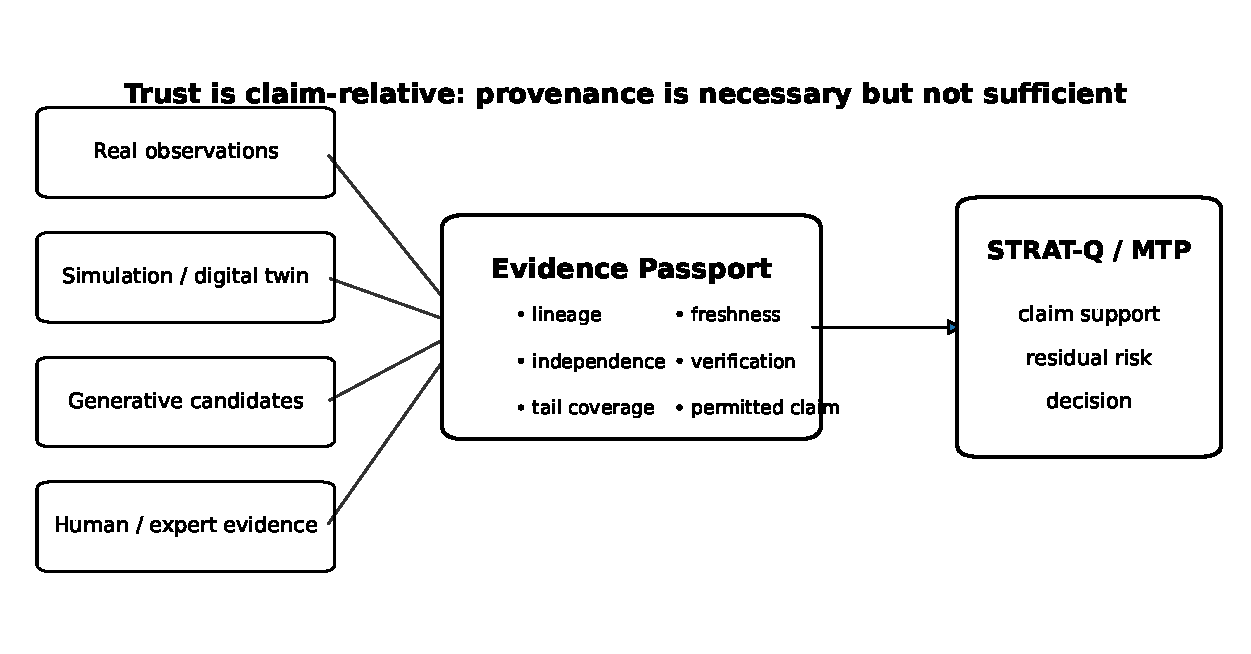
\includegraphics[width=0.95\textwidth]{figures/evidence_passport.pdf}
\caption{Evidence Passport connecting data provenance to STRAT-Q decisions.}
\label{fig:evidence-passport}
\end{figure}

Minimum fields are:

\begin{longtable}{p{0.23\textwidth}p{0.67\textwidth}}
\toprule
\textbf{Field} & \textbf{Meaning} \\
\midrule
Identity and version & Stable dataset or evidence identifier, schema version, timestamps \\
Origin class & Real observation, simulation, transformed real, generative, human review \\
Parent lineage & Parent datasets, generators, model versions, prompts, seeds, transformations \\
Generation depth & Number of generative steps since the last independent real anchor \\
Sampling policy & Temperature, top-$p$, top-$k$, rejection criteria, filtering \\
Oracle & How the expected result or validity was established \\
Verifier & Identity, independence, calibration, thresholds, false acceptance/rejection evidence \\
Freshness & Temporal, software-version, causal and distributional freshness \\
Tail coverage & Regimes covered, omitted, and intentionally oversampled \\
Permitted use & Training, exploration, regression, qualification, certification, or prohibited use \\
Supported claim & Exact claim and scope for which the evidence is relevant \\
Review status & Draft, automated-checked, expert-reviewed, approved, superseded, revoked \\
\bottomrule
\end{longtable}

\subsection{Verifiable Credentials are necessary but insufficient}

The W3C Verifiable Credentials model can establish issuer identity, integrity, status, and machine-verifiable presentation \citep{w3cvc2025}. It does not automatically establish that the content is true, current, representative, or sufficient for a decision.

We distinguish:

\begin{enumerate}[leftmargin=*]
  \item \textbf{Cryptographic verifiability:} who signed what and whether it changed;
  \item \textbf{Epistemic strength:} how reliable, independent, fresh and representative the evidence is;
  \item \textbf{Decision relevance:} whether it supports the specific claim under consideration.
\end{enumerate}

A strong signature can protect a weak dataset. Conversely, a real observation can be weak evidence if collection is biased or the deployment system has changed.

\subsection{Freshness is multidimensional}

Freshness should include:

\paragraph{Temporal freshness.} How long ago was the evidence created?

\paragraph{Version freshness.} Does it apply to the current software, model, sensor, architecture, or policy version?

\paragraph{Causal freshness.} Are the mechanisms that generated the evidence still active?

\paragraph{Distributional freshness.} Is
\[
d(P_{\mathrm{evidence}},P_{\mathrm{deploy}})
\]
within an acceptable bound?

\paragraph{Generational freshness.} How many synthetic transformations separate the evidence from an independent anchor?

A dataset generated yesterday can be generationally stale if it descends from multiple recursive teachers trained on obsolete data.

\subsection{Residual risk decomposition}

The MTP should distinguish uncertainty inside covered regimes from uncertainty due to absent regimes. A useful decomposition is
\[
R_{\mathrm{res}}
=R_{\mathrm{tested}}
+R_{\mathrm{missing}}
+R_{\mathrm{oracle}}
+R_{\mathrm{drift}}
+R_{\mathrm{dependence}}.
\]

\begin{itemize}[leftmargin=*]
  \item $R_{\mathrm{tested}}$: remaining failure risk in tested regimes;
  \item $R_{\mathrm{missing}}$: probability-weighted impact of regimes not covered;
  \item $R_{\mathrm{oracle}}$: uncertainty that expected outcomes or labels are wrong;
  \item $R_{\mathrm{drift}}$: mismatch between evidence and current deployment;
  \item $R_{\mathrm{dependence}}$: overconfidence caused by correlated evidence.
\end{itemize}

Synthetic testing often reduces $R_{\mathrm{tested}}$ efficiently. It can leave $R_{\mathrm{missing}}$ unchanged or even hidden.

\subsection{Probabilistic MTP integration}

The companion probabilistic MTP programme models incident probability as a distribution rather than a score. A simple Bayesian logistic model is
\[
\Prob(Y=1\mid X,w)
=\sigma(w^\top X+b),
\qquad
w\sim\mathcal N(\mu,\Sigma_w).
\]
The posterior is updated from test, defect, and production evidence. Synthetic-data lineage should enter either as covariates, hierarchical source effects, or likelihood weights. For source class $s$,
\[
y_j\sim\mathrm{Bernoulli}(p_j),
\qquad
\mathrm{logit}(p_j)=w^\top x_j + \alpha_{s_j},
\]
with source-specific uncertainty on $\alpha_s$.

A more explicit robust model can introduce latent label correctness $z_j$:
\[
\Prob(y_j^{\mathrm{obs}}\mid y_j^{\mathrm{true}},s_j)
\]
and infer source-specific false-label rates. This is preferable to treating a million pseudo-labels as perfect Bernoulli observations.

\subsection{Test-effort optimisation}

Let risk component $R_i^0$ be reduced by test effort $u_i$:
\[
R_i(u_i)=R_i^0e^{-\beta_i u_i}.
\]
Testing cost is
\[
C_{\mathrm{test}}(u)=\sum_i c_i u_i,
\]
and expected incident loss is
\[
C_{\mathrm{incident}}(u)
=L\sum_iR_i^0e^{-\beta_i u_i}.
\]
The optimiser solves
\[
\min_{u\ge0}
\sum_i c_i u_i
+L\sum_iR_i^0e^{-\beta_i u_i},
\]
subject to budget, calendar and resource constraints.

Synthetic data changes $\beta_i$: it may make a test category cheaper or more efficient, but only for the regimes it validly covers. We therefore replace $\beta_i$ by a posterior conditioned on evidence provenance:
\[
\beta_i\sim p(\beta_i\mid D_{\Real},D_{\Syn},V,\text{lineage}).
\]

The stopping condition remains marginal:
\[
c_i
=L R_i^0\beta_i e^{-\beta_i u_i},
\]
but uncertainty in $\beta_i$, missing-tail risk, and verification cost must be included.

\subsection{Four economic uses of test data}

A test-data budget can purchase four different things:

\begin{enumerate}[leftmargin=*]
  \item \textbf{Densification:} more confidence in an already-covered regime;
  \item \textbf{Extension:} entry into a missing or rare regime;
  \item \textbf{Refresh:} replacement of stale evidence;
  \item \textbf{Verification:} improvement of the oracle or synthetic-data reliability.
\end{enumerate}

These investments have different marginal values. The optimal test programme should choose among them rather than merely increasing execution count.

\subsection{Watermarking and provenance}

Watermarking can help detect probable synthetic origin. It does not establish truth or usefulness. A robust chain is:
\[
\text{watermark/detection}
\rightarrow
\text{provenance record}
\rightarrow
\text{credential}
\rightarrow
\text{evidence assessment}
\rightarrow
\text{decision}.
\]

The MTP should not infer ``synthetic means weak'' or ``real means strong.'' It should infer source-specific uncertainty and claim relevance.

\subsection{Reviewer and consolidation process}

Consolidation must preserve meaningful disagreement. A good evidence bundle contains:
\[
(\text{claim},\text{support},\text{contradictions},\text{scope},\text{confidence},\text{residual uncertainty}).
\]
It should not average away minority regimes. Reviewer actions should be versioned and themselves auditable.

\begin{keyidea}
Test Data Governance becomes part of the safety case. It documents not only what data exist, but why those data are allowed to reduce a specific residual risk.
\end{keyidea}

\section{Connections to companion studies}

\subsection{Probabilistic machine learning and the MTP}

The companion probabilistic MTP work proposes replacing static qualitative risk labels with posterior distributions, continuous Bayesian updates, and decision analysis. The synthetic-data lecture adds a missing qualification: likelihood terms are only as strong as the data-generating and labeling processes that created them.

A posterior can become overconfident if synthetic or duplicated observations are treated as independent. Hence probabilistic modelling must include data lineage and effective sample size, not only parameter uncertainty.

\subsection{Filtering and machine learning on manifolds}

The companion survey on filtering and machine learning on Riemannian manifolds and Lie groups emphasizes that state variables, covariance matrices, orientations and structured parameters may live on nonlinear spaces rather than ordinary Euclidean vectors \citep{labsir2026filtering}. This matters for the present study in three ways.

\paragraph{Geometric drift.} Recursive synthetic data may contract not only scalar variance but also the occupied region of a manifold. Euclidean averages can hide the loss of modes or violate constraints.

\paragraph{Uncertainty as an SPD object.} Covariance matrices lie on the manifold of symmetric positive definite matrices. Synthetic lineage can change both mean estimates and uncertainty geometry. Comparing covariances with Euclidean subtraction may be misleading.

\paragraph{Dynamic filtering.} Real anchors, synthetic predictions and verifier observations can be treated as sequential measurements of a latent system state. A geometric filter may update that state while respecting constraints.

A conceptual state is
\[
X_t\in\mathcal M,
\]
with dynamics
\[
X_{t+1}=F(X_t,u_t,\eta_t),
\]
and evidence
\[
Y_t=H(X_t,s_t,\nu_t),
\]
where source class $s_t$ affects observation noise. For MMALS, $X_t$ may include host ecology, route geometry, memory covariance, and goal state.

\subsection{Scientific machine learning and structure preservation}

The engineering-AI companion material stresses physics-informed and structure-preserving learning. The synthetic-data result provides a data-side counterpart. Structure can be lost through the training distribution even when the architecture contains the right inductive bias.

A system can therefore fail in two ways:

\begin{enumerate}[leftmargin=*]
  \item the model class violates physical or geometric constraints;
  \item the data pipeline removes the regimes needed to identify or preserve those constraints.
\end{enumerate}

For digital twins and scientific ML, synthetic simulation is especially valuable, but model-form error and calibration to real measurements must be explicit. More simulations of a biased simulator estimate the simulator more precisely, not the physical world.

\subsection{Continual learning}

Model collapse and catastrophic forgetting are related but distinct.

\begin{longtable}{p{0.23\textwidth}p{0.33\textwidth}p{0.34\textwidth}}
\toprule
\textbf{Phenomenon} & \textbf{Primary mechanism} & \textbf{Typical intervention} \\
\midrule
Catastrophic forgetting & Parameter updates overwrite earlier functions & Replay, regularization, modularity, isolation \\
Distributional unlearning & Training stream no longer contains skill-supporting cases & Restore or synthesize the missing regimes \\
Recursive label collapse & Previous predictions become future truth & Independent labels, verifier, lineage weighting \\
Functional route collapse & Rare hosts/routes lose access and gradient & Causal tail audit, real anchors, dynamic exploration \\
\bottomrule
\end{longtable}

MMALS must measure all four separately. Strong retention on previously replayed tasks does not prove preservation of unseen compositional support.

\subsection{Biometric synthetic data}

In biometrics, synthetic images can help when real identity data are scarce or sensitive. However, visual realism is insufficient. A fingerprint or face generator must be evaluated for:

\begin{itemize}[leftmargin=*]
  \item identity diversity and intra-identity diversity;
  \item sensor and acquisition-condition coverage;
  \item biometric quality distributions;
  \item non-memorization and privacy leakage;
  \item matcher utility on independent real data;
  \item long-tail failure modes;
  \item non-correspondence claims under defined thresholds.
\end{itemize}

Recursive GAN or diffusion training can amplify mode collapse and generator artefacts. The correct pattern is targeted generation plus independent matcher, simulator, quality, and privacy evaluation. Synthetic data should augment a governed real anchor, not silently replace it.

\subsection{Claim, protocol, and metric verification}

The planned MMALS verifier stack maps directly to the lecture:

\begin{itemize}[leftmargin=*]
  \item \textbf{Metric evaluator:} computes continuous evidence, not only exact-match success;
  \item \textbf{Protocol verifier:} checks that the experiment is independent, correctly split, seeded, and comparable;
  \item \textbf{Claim verifier:} checks whether the measured evidence actually supports the wording of the claim.
\end{itemize}

Verifier outputs should not become unchallenged truth. Their calibration, false acceptance, false rejection, and domain of validity are first-class evidence.

\section{Experimental programme and reproducibility roadmap}

\subsection{A staged research programme}

The lecture should not directly trigger a large end-to-end MMALS redesign. It should generate a ladder of falsifiable experiments.

\begin{figure}[H]
\centering
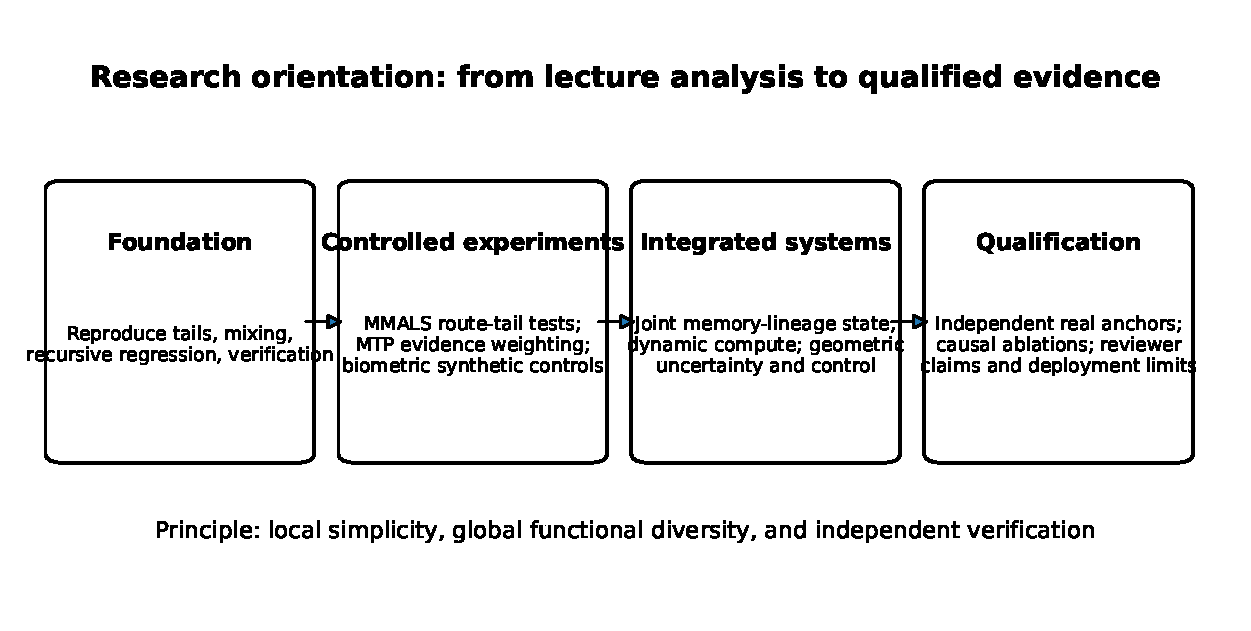
\includegraphics[width=0.97\textwidth]{figures/research_roadmap.pdf}
\caption{Proposed research roadmap.}
\label{fig:roadmap}
\end{figure}

\subsection{Stage 0: reproduce the mathematical mechanisms}

The repository includes lightweight simulations of:

\begin{enumerate}[leftmargin=*]
  \item Hutter scaling under a power-law input distribution;
  \item chopped-tail error floors;
  \item real/synthetic mixing under scarcity;
  \item recursive relabeling;
  \item verifier-based candidate selection.
\end{enumerate}

The objective is not to reproduce every constant from the papers. It is to verify the qualitative signatures:

\begin{itemize}[leftmargin=*]
  \item power-law decrease;
  \item cutoff-dependent plateau;
  \item increased benefit under real-data scarcity;
  \item generational drift under pseudo-label recursion;
  \item recovery when verification enriches correct examples.
\end{itemize}

\subsection{Stage 1: MMALS synthetic-route benchmark}

Construct a controlled problem with known functional regimes. For example:

\begin{itemize}[leftmargin=*]
  \item regime $R_1$: one host is sufficient;
  \item regime $R_2$: a different host is superior;
  \item regime $R_3$: sequential collaboration is necessary;
  \item regime $R_4$: memory is useful;
  \item regime $R_5$: old memory is misleading and must be overridden.
\end{itemize}

Train an initial MMALS version on independently labeled routes, then generate recursive route labels for later versions.

\paragraph{Treatments.}
\begin{enumerate}[leftmargin=*]
  \item real/oracle traces only;
  \item recursive synthetic traces only;
  \item fixed real anchor plus synthetic traces;
  \item accumulated fresh real traces plus synthetic traces;
  \item verified synthetic candidate routes;
  \item lineage-aware consolidation;
  \item dual reconstructive/compiled memory;
  \item state-dependent temperature versus fixed temperature.
\end{enumerate}

\paragraph{Metrics.}
\begin{itemize}[leftmargin=*]
  \item task accuracy and calibrated loss;
  \item final average retention and forgetting;
  \item functional tail coverage;
  \item route entropy and dominance;
  \item host ablation impact;
  \item route-swap degradation;
  \item candidate-permutation sensitivity;
  \item cost per solved input;
  \item number of iterations to convergence;
  \item abstention quality;
  \item synthetic lineage depth;
  \item recovery delay after real anchors are reintroduced.
\end{itemize}

\subsection{Stage 2: verifier bootstrap}

For each input, generate $K$ candidate routes. Let an independent oracle or task residual rank them. Compare:

\begin{itemize}[leftmargin=*]
  \item teacher top-1 route;
  \item oracle best-of-$K$ route;
  \item learned verifier top-1 route;
  \item student trained on accepted routes.
\end{itemize}

A strong result would show:
\[
Q(\text{student}) > Q(\text{teacher top-1})
\]
on an independent real evaluation set, while maintaining or improving functional tail coverage.

The verifier must be audited with:
\[
\phi=\Prob(\text{accept}\mid\text{valid}),
\qquad
\psi=\Prob(\text{accept}\mid\text{invalid}),
\]
stratified by regime and rarity.

\subsection{Stage 3: probabilistic MTP benchmark}

Create a project-level dataset with:

\begin{itemize}[leftmargin=*]
  \item contract and technical-offer features;
  \item preliminary design and dependency structure;
  \item TRL or maturity estimates;
  \item expected margins and resource constraints;
  \item proposed test categories and effort;
  \item defects discovered and production incidents;
  \item source lineage of each observation and test case.
\end{itemize}

Compare four estimators:

\begin{enumerate}[leftmargin=*]
  \item all evidence treated as independent and real;
  \item source-weighted Bayesian model;
  \item hierarchical model with source-specific noise;
  \item lineage-aware model with effective sample-size correction.
\end{enumerate}

Evaluate calibration, posterior coverage, decision regret, residual-risk estimates, and stability under synthetic-data contamination.

\subsection{Stage 4: geometric extension}

Represent covariance, route similarity, or host-state structure on an appropriate manifold. Candidate directions include:

\begin{itemize}[leftmargin=*]
  \item SPD geometry for uncertainty and covariance states;
  \item Stiefel manifolds for learned subspaces;
  \item graph manifolds for dependency or host ecology;
  \item Lie-group state spaces for controlled transformations.
\end{itemize}

The research question is not whether geometric methods are more sophisticated. It is whether they preserve functional distinctions, improve filtering, or provide intrinsic uncertainty bounds that the Euclidean model misses.

\subsection{Ablation discipline}

Every claimed benefit must be compared to the simplest alternative:

\begin{longtable}{p{0.30\textwidth}p{0.58\textwidth}}
\toprule
\textbf{Claimed mechanism} & \textbf{Minimum baseline} \\
\midrule
Synthetic generation & Retrieval or replay of real examples under the same budget \\
Complex router & Four-parameter or linear softmax router \\
Geometry & Euclidean representation with matched dimensions and parameters \\
Memory synthesis & Exact reconstructive replay \\
Verifier & Ground-truth oracle and random/score-only filters \\
Host specialization & Equal-parameter single-host and shared-host controls \\
Dynamic compute & Fixed-depth and fixed-active-host baselines \\
Lineage weighting & Unweighted mixture and simple real/synthetic indicator \\
\bottomrule
\end{longtable}

\subsection{Claim ladder}

The experimental programme should use a claim ladder.

\begin{description}[leftmargin=3.5cm,style=nextline]
  \item[Level 0: Pipeline.] Code runs and records lineage.
  \item[Level 1: Association.] Route distributions change under recursive data.
  \item[Level 2: Functional effect.] Tail loss correlates with rare-regime degradation.
  \item[Level 3: Causality.] Ablations and controlled interventions identify necessary mechanisms.
  \item[Level 4: Generalisation.] Results replicate across seeds, tasks and backbone families.
  \item[Level 5: Deployment value.] The intervention improves verified performance or risk under realistic cost.
\end{description}

\subsection{Repository outputs}

The accompanying package contains:

\begin{itemize}[leftmargin=*]
  \item this LaTeX source and compiled PDF;
  \item original vector figures;
  \item scripts to regenerate figures and toy datasets;
  \item a tutorial notebook;
  \item CSV outputs;
  \item a research roadmap;
  \item an MMALS orientation note;
  \item a STRAT-Q/Test Data Governance orientation note;
  \item citation and licensing metadata.
\end{itemize}

\section{Conclusion: beyond raw scaling}

Julia Kempe's lecture presents a sobering but constructive view of the synthetic-data age. Scaling laws were observed under assumptions about data distributions that recursive model-generated corpora can violate. The consequences include altered exponents, error floors, lost skills, recursive label bias, delayed recovery, and verifier-dependent phase transitions.

The lecture does not imply that synthetic data should be rejected. It establishes a more precise doctrine:

\begin{enumerate}[leftmargin=*]
  \item synthetic data are most useful when real data are scarce or when they target otherwise inaccessible regimes;
  \item synthetic volume cannot recover support that the generator never produces;
  \item recursive pseudo-labels require independent corrective signals;
  \item real data, accumulation, and verification can change the asymptotic outcome;
  \item data curation becomes part of model architecture and risk governance.
\end{enumerate}

For MMALS, the deepest translation is that an adaptive system must preserve the conditions of future surprise. A route should not become dominant merely because it generated most of the replay. A memory should not become true because several system generations repeated it. A rare host should not be maintained for diversity theatre, but neither should it disappear before its causal value is tested.

The target architecture is therefore:
\[
\boxed{
\text{local simplicity}
+\text{global functional diversity}
+\text{independent verification}
+\text{lineage-aware memory}
}
\]

For STRAT-Q and probabilistic MTP, evidence must be discounted by dependence, lineage, freshness, oracle uncertainty, and missing-tail risk. The number of tests is not the number of independent proofs. A cryptographically verifiable credential is an authenticity layer, not an epistemic conclusion.

For engineering and scientific machine learning, simulation and generation remain powerful. Their role is to propose, explore, densify, and stress. Real measurements and validated constraints remain necessary to correct model-form error.

\begin{keyidea}
The next era is not literally ``beyond scaling'' in the sense that scale no longer matters. It is beyond the belief that scale is sufficient. What must scale is verified, diverse, fresh, decision-relevant functional support.
\end{keyidea}

\appendix
\section{Notation and glossary}

\begin{longtable}{p{0.18\textwidth}p{0.72\textwidth}}
\toprule
\textbf{Symbol / term} & \textbf{Meaning} \\
\midrule
$T$ & Number of training samples \\
$d,N$ & Model size or parameter capacity \\
$\beta$ & Tail exponent in a Zipf-like distribution \\
$k$ & Synthetic-data cutoff rank or effective support size \\
$E_{\mathrm{test}}$ & Test error under the target distribution \\
$T_{\Real},T_{\AI}$ & Numbers of real and AI-generated examples \\
$\tau$ & Sampling or routing temperature \\
$\phi$ & Verifier true acceptance probability \\
$\psi$ & Verifier false acceptance probability \\
$w_0$ & Ground-truth regression parameter \\
$\widehat w_g$ & Parameter learned at synthetic generation $g$ \\
Functional tail & Rare but valid tasks, routes, hosts, or regimes \\
Tail cutting & Assigning zero probability to part of the valid support \\
Tail narrowing & Retaining support but reducing rare-event probabilities \\
Model collapse & Generic term requiring a more precise diagnosis \\
Grokking & Delayed generalisation after an apparent plateau or overfit phase \\
Evidence Passport & Provenance and claim-relevance metadata for evidence \\
Real anchor & Independent observation capable of correcting synthetic recursion \\
Reconstructive memory & Auditable storage of detailed routes and intermediate states \\
Compiled memory & Compressed reusable functional knowledge \\
FTC & Functional Tail Coverage \\
\bottomrule
\end{longtable}

\section{Claim-to-evidence matrix}

\begin{longtable}{p{0.28\textwidth}p{0.27\textwidth}p{0.35\textwidth}}
\toprule
\textbf{Claim} & \textbf{Required evidence} & \textbf{Insufficient evidence} \\
\midrule
Synthetic data improve training & Gain on independent real evaluation under matched budget & Gain only on self-generated validation data \\
MMALS self-organises & Reproducible functional differentiation and causal route effects & Visually interesting routing or high entropy \\
Hosts specialise & Host-specific contribution, ablation impact, stable regime association & Unequal activation frequency alone \\
Memory generalises & Improvement on unseen variants and compositions & Exact replay success \\
Verifier prevents collapse & Calibrated acceptance and preserved rare-regime coverage & High average verifier accuracy only \\
More tests reduce residual risk & Posterior or empirical reduction in decision-relevant failure risk & Increased execution count or pass rate \\
Credential is trustworthy & Integrity plus independent epistemic assessment & Valid signature alone \\
Geometry is necessary & Matched Euclidean baseline and intrinsic benefit & Use of manifold terminology or visualization \\
Dynamic compute adapts & Cost increases with verified difficulty and decreases on simple cases & Variable runtime without quality/cost control \\
\bottomrule
\end{longtable}

\section{Reproducibility notes}

\subsection{Generated figures}

All conceptual figures in this report are generated by \texttt{code/generate\_figures.py}. CSV files under \texttt{data/} contain the plotted toy values. These are educational simulations and not reproductions of the original paper experiments.

\subsection{Tutorial notebook}

The notebook \texttt{notebooks/synthetic\_data\_scaling\_tutorial.ipynb} provides executable cells for:

\begin{itemize}[leftmargin=*]
  \item power-law distributions;
  \item Hutter missing mass;
  \item chopped-tail scaling;
  \item mixed real/synthetic data;
  \item recursive ridge-style relabeling;
  \item verifier filtering;
  \item a conceptual MMALS route-collapse simulation.
\end{itemize}

\subsection{Limits of reproduction}

The package does not include copyrighted lecture slides, model weights, WikiText-103, or the large transformer experiments from the cited papers. It provides links and references for the original materials. Exact reproduction of the published results requires the authors' code, datasets, model versions, and computational resources.

\subsection{Suggested repository name}

\texttt{synthetic-data-scaling-mmalls}

Suggested description:

\begin{quote}
A multilevel analysis of Julia Kempe's synthetic-data and model-collapse lecture, with reproducible scaling-law tutorials and research orientations for MMALS, STRAT-Q, probabilistic MTP, and Test Data Governance.
\end{quote}


\bibliographystyle{plainnat}
\bibliography{references}

\end{document}
